% TRABALHOS RELACIONADOS--------------------------------------------------------

\chapter{TRABALHOS RELACIONADOS}
\label{chap:trabalhosrelacionados}

\section{Automação e Controle em Sistema de Aproveitamento de Água da Chuva para 
Fins Não Potáveis}

\textbf{Autora:} Lilia Rodrigues Lucas Magalhães
\vspace{\onelineskip}

Este trabalho de conclusão de curso realizado por Lilia Rodrigues Lucas Magalhães pelo Centro Universitário de Brasília - UniCEUB apresenta uma protosta muito semelhante ao trabalho a ser desenvolvido.

A ideia deste projeto foi demonstrar o funcionamento automatizado de um sistema (representado na \autoref{fig:trab_rel_01} ) de aproveitamento de água de chuva por meio da elaboração de um protótipo composto pela maquete de um banheiro, confeccionada em madeira, juntamente com três reservatórios em acrílico. Esse cenário representa o sistema de distribuição de água de chuva dentro de uma residência e destina-se à utilização em descarga sanitária.

\begin{figure}[H]
	\centering
	\caption{Corte Esquemático do Sistema de Aproveitamento Proposto.}
	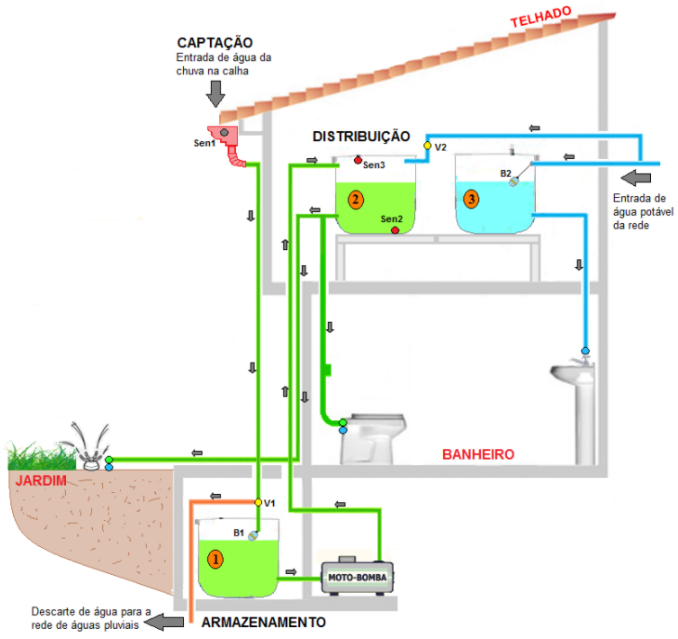
\includegraphics[width=0.7\textwidth]{figuras/trabalhos_relacionados/fig01.png}
	\label{fig:trab_rel_01}
\end{figure}

O projeto, implementado fisicamente e virtualmente no \textit{software Proteus} (\autoref{fig:trab_rel_02}), foi baseado para uma aplicação sem a conexão com redes remotas e utilizando componentes eletrônicos mais simples, como portas analógicas. O microcontrolador utilizado foi o \textit{Philips 80C552} acoplado ao Kit \textit{CW 552}, considerado defasado atualmente. Esse trabalho fomentou a ideia da utilização de válvulas solenoides para direcionamento do fluxo de água, assim como métodos para medição de nível e uma abordagem sobre as rotinas de funcionamento do microcontrolador.

\begin{figure}[H]
	\centering
	\caption{Simulação elaborada no \textit{Software Proteus}.}
	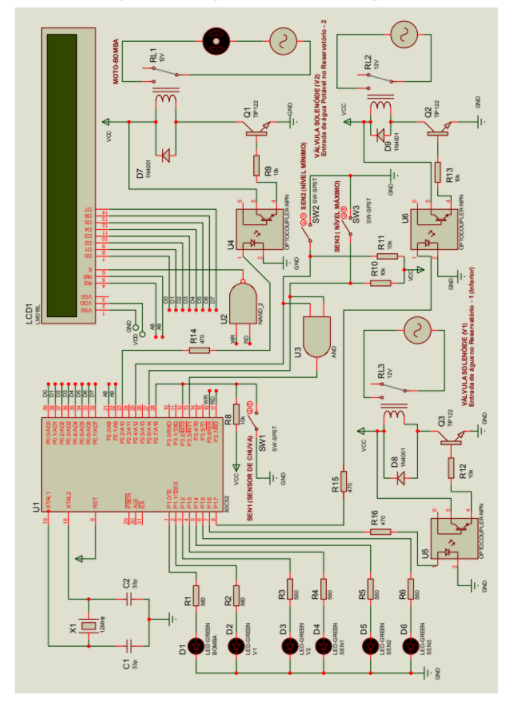
\includegraphics[width=0.5\textwidth, angle=-90]{figuras/trabalhos_relacionados/fig02.png}
	\label{fig:trab_rel_02}
\end{figure}

\begin{figure}[H]
	\centering
	\caption{Microcontrolador \textit{Philips 80C552} acoplado ao kit \textit{CW 552}.}
	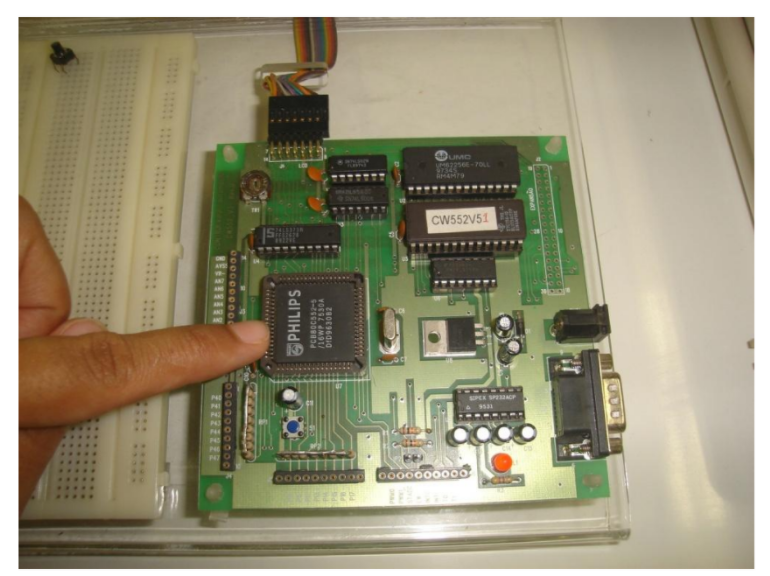
\includegraphics[width=0.5\textwidth]{figuras/trabalhos_relacionados/fig03.png}
	\label{fig:trab_rel_03}
\end{figure}

\newpage

\section{Automação residencial Usando protocolo \textit{MQTT}, \textit{NODE-RED} e \textit{Mosquitto Broker} com \textit{ESP32} e \textit{ESP8266}}

\textbf{Autor:} Victor Ferreira Martins
\vspace{\onelineskip}

Este trabalho de conclusão de curso desenvolvido por Victor Ferreira Martins teve o objetivo de propor uma solução de automação residencial que fosse capaz de integrar três diferentes sistemas em uma casa: monitoramento de temperatura, alarmes de segurança e acionamento de iluminação e tomadas. O objetivo dessa integração foi ajudar a alcançar três dos grandes objetivos da automação residencial: conforto, segurança e economia de energia.
Como caraterísticas importantes destacam-se: a utilização do protocolo\textit{ MQTT} para comunicação através do \textit{Mosquitto Broker}, assim como o uso da ferramenta de programação visual \textit{Node-RED} e dos microcontroladores \textit{ESP32} e \textit{ESP8266}.

Em relação ao trabalho pode-se abstrair os seguintes dados:

\begin{enumerate}
	\item A utilização do protocolo \textit{MQTT}, por meio do \textit{Broker Mosquitto} em conjunto com os microcontroladores da \textit{ESPRESSIF};
	\item A utilização de diversos sensores, validando que a conexão e transferência de dados através do protocolo \textit{MQTT};
	\item Uma abordagem para a organização dos tópicos \textit{MQTT} (\autoref{tab:tabela_topicos}), definindo dispositivos de publicação (\textit{publishers}) e de inscrição (\textit{subscribes});
	\item A utilização do \textit{Node-RED} como agente de interfaceamento do projeto (\autoref{fig:trab_rel_01}).
\end{enumerate}

\begin{figure}[H]
	\centering
	\caption{Visão geral do projeto.}
	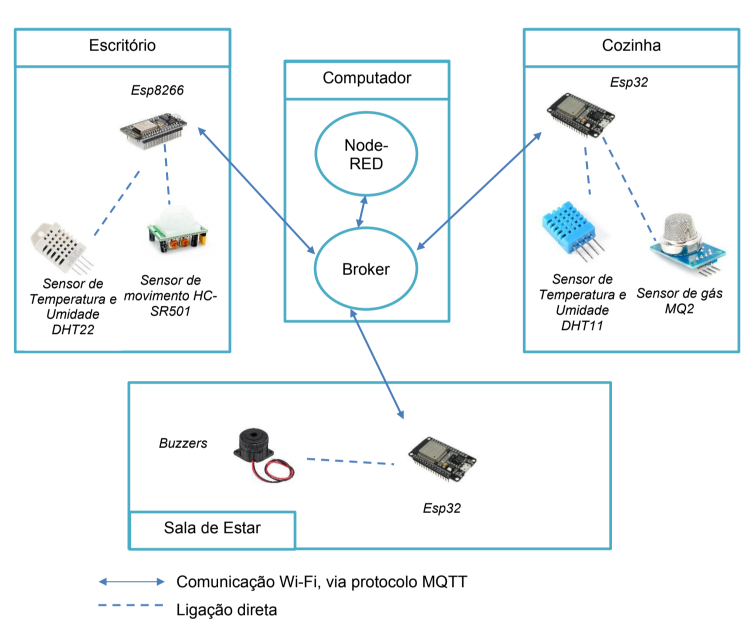
\includegraphics[width=0.8\textwidth]{figuras/trabalhos_relacionados/fig04.png}
	\label{fig:trab_rel_04}
\end{figure}

\begin{figure}[H]
	\centering
	\caption{Visualização da interface desenvolvida no \textit{Node-RED} para receber entradas do usuário e mostrar dados dos sensores.}
	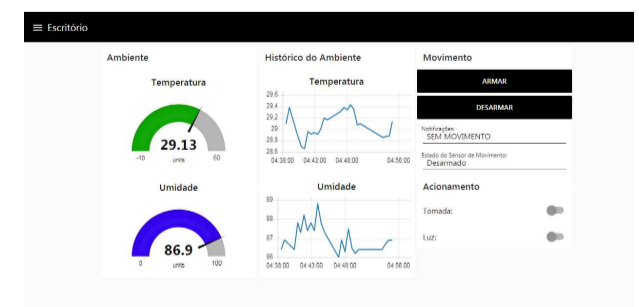
\includegraphics[width=0.8\textwidth]{figuras/trabalhos_relacionados/fig05.png}
	\label{fig:trab_rel_05}
\end{figure}

\begin{table}[H]
	\centering
	\small
	\caption{Organização dos tópicos \textit{MQTT}.}
	\begin{tabular}{c|c|c}
		\hline
		\textbf{Dispositivo} & \textbf{Inscrição} & \textbf{Publicação} \\ \hline
		\multirow{4}{*}{\begin{tabular}[c]{@{}c@{}}ESP8266\\ \\ (Escritório)\end{tabular}} & \multirow{2}{*}{casa/escritório/esp8266/movimento} & casa/escritório/esp8266/temperatura \\ \cline{3-3} 
		&  & casa/escritório/esp8266/umidade \\ \cline{2-3} 
		& casa/escritório/esp8266/tomada & \begin{tabular}[c]{@{}c@{}}casa/escritório/esp8266/movimento/\\ estado\end{tabular} \\ \cline{2-3} 
		& casa/escritório/esp8266/luz & \begin{tabular}[c]{@{}c@{}}casa/escritório/esp8266/movimento/\\ notificação\end{tabular} \\ \hline
		\multirow{4}{*}{\begin{tabular}[c]{@{}c@{}}ESP32\\ (Cozinha)\end{tabular}} & casa/esp32/cozinha/fumaça & casa/cozinha/esp32/temperatura \\ \cline{2-3} 
		& \begin{tabular}[c]{@{}c@{}}casa/cozinha/esp32/\\ tomada\end{tabular} & casa/cozinha/esp32/umidade \\ \cline{2-3} 
		& \multirow{2}{*}{casa/cozinha/esp32/luz} & casa/cozinha/esp32/fumaça/estado \\ \cline{3-3} 
		&  & casa/cozinha/esp32/fumaça/notificação \\ \hline
		\multirow{2}{*}{\begin{tabular}[c]{@{}c@{}}ESP32\\ (Sala de estar)\end{tabular}} & casa/escritório/esp8266/notificação & \multirow{2}{*}{-} \\ \cline{2-2}
		& casa/cozinha/esp32/notificação &  \\ \hline
	\end{tabular}
	\label{tab:tabela_topicos}
\end{table}

\newpage

\section{Desenvolvimento de plataformas embarcadas aplicadas a implementação de \textit{Smart Buildings} com base no \textit{framework SmartLVGrid}}

\textbf{Autor:} Rubens de Andrade Fernandes
\vspace{\onelineskip}

Este trabalho de conclusão de curso desenvolvido por Rubens de Andrade Fernandes pela Universidade do Estado do Amazonas concentrou-se no desenvolvimento de algorítimos para \textit{software} embarcado e dispositivos
de \textit{hardware}, associados a plataformas microcontroladas e microprocessadas, com o objetivo de realizar a convergência \textit{smart building} em sistemas de iluminação e medição de energia elétrica sem recursos de automação, comunicação e controle.

Os pontos relevantes deste trabalho em relação à para implementação deste TCC estão na criação de rotinas de cadastro geradas exclusivamente pelos microcontroladores \textit{ESP32} utilizados (Figura 5.6). 

\begin{figure}[H]
	\centering
	
	\caption{Configuração dos dispositivos}
	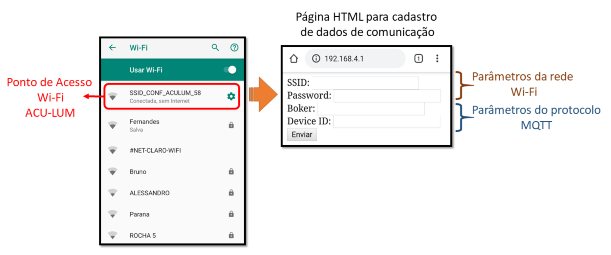
\includegraphics[width=0.8\textwidth]{figuras/trabalhos_relacionados/fig06.png}
	\label{fig:trab06}
\end{figure}

Essa rotina de cadastro faz com que o microcontrolador forneça um ponto de acesso local possibilitando qualquer o acesso de qualquer dispositivo. Ao realizar uma conexão através de um computador ou \textit{smartphone}, por exemplo, o usuário pode informar dados de cadastro como para o dispositivo operar em rede.

O segundo ponto que se pode destacar desse trabalho foi a criação de bibliotecas que auxiliam na operação do microcontrolador como demonstrado na tabela abaixo. 

\begin{table}[H]
	\centering
	\small
	\caption{Bibliotecas implementadas para elaboração do \textit{firmware}}
	\begin{tabular}{cc}
		\hline
		Bibliotecas & Descrição \\ \hline
		DriverAcuLum & \begin{tabular}[c]{@{}c@{}}Utilizada para implementar os métodos referentes\\  as DRFs a serem executadas\end{tabular} \\
		DriverMQTT & \begin{tabular}[c]{@{}c@{}}Utilizada para garantir confiabilidade e \\ segurança no uso do protocolo MQTT\end{tabular} \\
		DriverWIFI & \begin{tabular}[c]{@{}c@{}}Utilizada para garantir uma conexão mais estável, \\ robusta e segura na rede Wi-Fi\end{tabular} \\
		SaveData & \begin{tabular}[c]{@{}c@{}}Utilizada para armazenar os parâmetros do ACU-LUM \\ na EEPROM do ESP32\end{tabular} \\ \hline
	\end{tabular}
	\label{tab:my-table}
\end{table}

Outro ponto importante foi a confecção dos módulos propostos, utilizando técnicas de modelagem 3D para visualização \textit{PCB's} e a realização de soldagem e inserção de componentes.

\begin{figure}[H]
	\centering
	\label{fig:trab_rel_07}
	\caption{Comparação entre o \textit{layout 3D} e o dispositivo físico montado}
	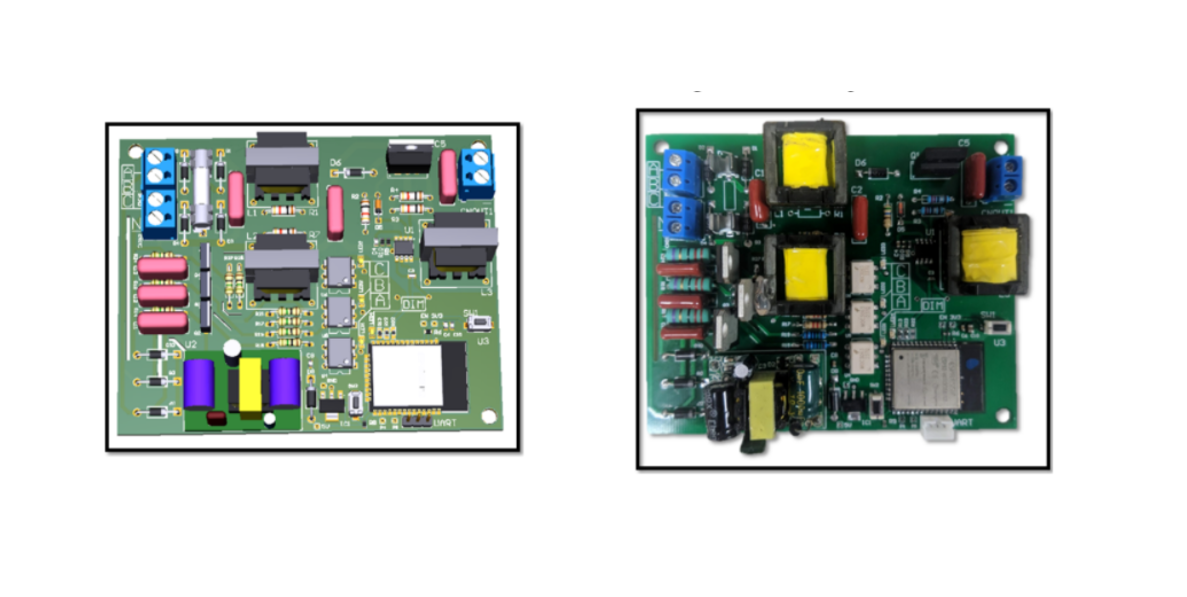
\includegraphics[width=0.5\textwidth]{figuras/trabalhos_relacionados/fig07.png}
	
\end{figure}



\section{Design, Implementation and Practical Evaluation of an IoT Home Automation System for Fog Computing Applications Based on \textit{MQTT} and \textit {ZigBee-WiFi}	Sensor Nodes}

\textbf{Autores:} Iván Froiz-Míguez, Tiago M. Fernández- Camaramés, Paula Fraga-Lamas e Luis Castedo
\vspace{\onelineskip}

Este artigo desenvolvido por membros do departamento de engenharia de computação, da Universidade da Coruña, Espanha, apresentou um estudo de caso e aplicação onde buscou-se unir duas tecnologias dentro das características da \textit{IoT}: \textit{WI-FI} e o protocolo \textit{ZigBee}. O protocolo \textit{ZigBee} é muito utilizado quando se tem a necessidade de uma comunicação à longas distâncias com um baixo consumo energético.

O trabalho apresentou a formulação de uma nova tecnologia: o \textit{ZiWi}, um \textit{HAS - Home Automation System} de computação em nuvem que preenche a lacuna entre dispositivos \textit{ZigBee} e \textit{Wi-Fi}, conectando sensores e atuadores perfeitamente para fazer uso de tais tecnologias em uma residência. O \textit{ZiWi} utiliza o \textit{Wi-Fi} para comunicação com atuadores já que, em geral, há a necessidade de estar continuamente operando e ouvindo comandos assíncronos. Enquanto o \textit{ZigBee} é aplicado para sensores porque é ideal para enviar dados em intervalos periódicos, a fim de economizar energia (já que muitos sistemas dependem de baterias). Além disso, o sistema se concentra no crescente mercado de \textit{IoT} e na utilização de sensores emergentes. Além disso, \textit{ZiWi} faz uso da computação em nuvem, paradigma para fornecer conectividade entre o usuário e os diferentes eletrodomésticos, não apenas
permitindo ao usuário controlá-los, mas também oferecendo a possibilidade dos dispositivos aprenderem com bancos de dados \textit{online}. Isso é alcançado
graças à natureza distribuída do \textit{ZiWi}: o hardware do controlador doméstico é mantido com o mínimo de execuções de tarefas em tempo real, delegando o processamento dos dados e as decisões em tempo não real para servidores em nuvem remotos.

Com a utilização o \textit{Wi-Fi}, o trabalho procurou integrar o protocolo \textit{MQTT} (como a figura de um dispositivo \textit{Broker}, a publicação e inscrição em tópicos) para dispositivos que trabalhavam com o protocolo \textit{ZigBee}. A técnica desenvolvida se tornou muito interessante para aplicações em trabalhos posteriores a esse TCC, como a utilização em ambientes mais isolados.

\begin{figure}[H]
	\centering
	\label{fig:trab_rel_08}
	\caption{Esquema para aplicação do protocolo \textit{ZiWi}}
	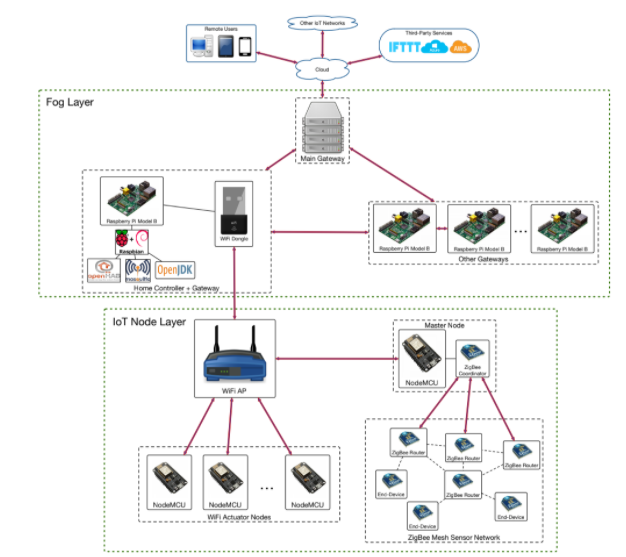
\includegraphics[width=1.0\textwidth]{figuras/trabalhos_relacionados/fig08.png}
	
\end{figure}
 